\scanpage{56}

$\rho=\rho_s,\ \rho'=\underset{\substack{\shortparallel\\\rho_{f'}^{-1}}}{\rho_f}$. Si $s\prec f$, on est dans le cas déjà traité dans a). Sinon, on a $s\prec f'$ donc

\deleted{\unsure{$\rho_s$} $(\rho_{f'},\rho_s,\rho_a)$ est un syst. de Schwartz canonique (où $a\in A$ est \unsure{choisi|défini} de façon que $(s,a,f')\in R^{+}$).}

\figure{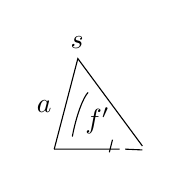
\begin{tikzpicture}[x=1cm,y=1cm]\draw(0,0)--(.30,1.15)--(1.12,.04);\draw(0,0)--(.83,0) (.9,0)--(1.12,-.01);\draw[thin](.70,-.04)--(.74,.12);\draw(.23,.16) .. controls (.28,.43) and (.37,.66) .. (.43,.72);\node[above] at (.29,1.15){$s$};\node[left] at (.09,.54){$a$};\node at (.55,.36){$f'$};\end{tikzpicture}}

\deleted{Donc $(\rho_s^{-1}\deleted{\unsure{^{2}}},\rho_{f'}^{-1}=\rho_f^{\deleted{\unsure{+}}},\rho_a^{-1}=\rho_a)=(\rho^{-1},\rho',\rho_a)$ est un syst. canonique. Donc \unsure{soit} $(\rho,\rho',\rho'')=\rho=\rho_s,\rho$}

Cela donne une seule autre possibilité comme position relative d'un él. d'ordre $4$ et d'un él. d'ordre $3$ qui ne commutent pas -- celui traité dans c) [type $(4,3,4)$] absurde. cqfd.

% archive sheet number: 55
